\documentclass[14pt]{extarticle}

\usepackage{enumitem}
\usepackage{calc}
\usepackage{tikz}
\usepackage{wrapfig}
\usepackage{graphicx}
\graphicspath{ {./images/} }
\usepackage{listings}
\usepackage{color}
\usepackage{textcomp}
\definecolor{listinggray}{gray}{0.9}
\definecolor{lbcolor}{rgb}{0.9,0.9,0.9}
\lstset{
	backgroundcolor=\color{lbcolor},
	tabsize=4,
	rulecolor=,
	language=bash,
  basicstyle=\scriptsize,
  upquote=true,
  aboveskip={1.5\baselineskip},
  columns=fixed,
	morekeywords={gcc, gdb, sudo, rm, chmod, chown, ln, ls, s, w, ln, vim, hexdump, z, o, while, do, done, echo},
  showstringspaces=false,
  extendedchars=true,
  breaklines=true,
  prebreak = \raisebox{0ex}[0ex][0ex]{\ensuremath{\hookleftarrow}},
  frame=single,
  showtabs=false,
  showspaces=false,
  showstringspaces=false,
  identifierstyle=\ttfamily,
  keywordstyle=\color[rgb]{0,0,1},
  commentstyle=\itshape\color{purple!40!black},
  stringstyle=\color[rgb]{0.627,0.126,0.941},
}
\lstdefinestyle{customc}{
  belowcaptionskip=1\baselineskip,
  breaklines=true,
  frame=L,
  xleftmargin=\parindent,
  language=C,
  showstringspaces=false,
  basicstyle=\footnotesize\ttfamily,
  keywordstyle=\bfseries\color{green!40!black},
  commentstyle=\itshape\color{purple!40!black},
  identifierstyle=\color{blue},
  stringstyle=\color{orange},
}
\lstdefinelanguage{sh}{
morekeywords={gcc, gdb, sudo, rm, chmod, chown, ln, ls, s, w, ln, vim, hexdump, z, o, while, do, done, echo},
sensitive=false
}
\newcommand{\inlinecode}[2]{\colorbox{lightgray}{\lstinline[language=#1]$#2$}}

\usetikzlibrary{trees}
\parskip=.9ex
\textwidth=7.0in
\textheight=9.0in
\oddsidemargin=-.25in
\topmargin=-.75in

\begin{document}

\title{Buffer Overflows Classic}

\author{Zane Durkin\\
    University of Idaho}
\begin{description}[leftmargin=!, labelwidth=\widthof{\bfseries Author(s) Name(s)}]
\item [Year and Semester] 2018 FALL
\item [Course Number] CS-336
\item [Course Title] Intro. to Information Assurance
\item [Work Number] LA-03
\item [Work Name] SQL Injection attack
\item [Work Version] Version 1
\item [Long Date] Sunday, 11 November 2018
\item [Author(s) Name(s)] Zane Durkin
\end{description}
\begin{abstract}
In this article I will be explaining in detail the Tasks I preformed during the SEED security lab3.
\end{abstract}

\setcounter{section}{-1}
\section{Lab environment}
The website will be running locally on the virtual machine. To access the web version of the site, I can visit http://www.SEEDLabSQLInjection.com on the VM's browser (this site is only available from within the VM). The host file is set to point this address to localhost, and Apache is set to display a local site at this address. The files for this site are located at /var/www/SQLInjection/ so I can see of the website is handling the data I pass to it.\cite{seed-sqlatk}.

\subsection{Apache configuration}
The VM comes with apache pre-configured to display this site properly at the given address. If any re-configuration is needed, it is important that I reload apache before the changes will take effect. This can be done with the command:
\cite{seed-sqlatk}.
\begin{lstlisting}[language=sh]
sudo service apache2 start
\end{lstlisting}
\subsection{Web application}
The website that will be exploited is a basic employee management application. The employees have two basic roles, either Administrator or Employee. The two roles are allowed different privileges, such as the ability to edit everyone's information, or just their own information. Through this application employees can login with a username and password, edit their data, and see information currently stored about them\cite{seed-sqlatk}.

\section{Task 1: Get familiar with SQL statements}
In order to understand how a SQL injection attack can work, I first need to learn about how to form SQL queries, and how they can be manipulated. To start I will log into the mysql console using root.
\begin{lstlisting}[language=sh]
mysql -u root -pseedubuntu
\end{lstlisting}
Now that I'm in the mysql console, I'll want to select a database to use. For this lab I'll be focusing on the Users database, so I'll use that one.
\begin{lstlisting}[language=sh]
mysql> use Users;
\end{lstlisting}
\begin{center}
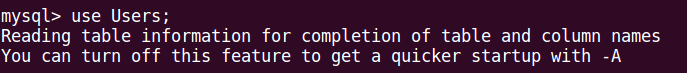
\includegraphics[width=.8\linewidth]{use-users}\\
\end{center}
Now that I have selected a database, mysql will know that when I wish to select or insert data I will mean to do so in the Users database. Since I haven't looked at this database before, I'll want to see what tables are in this database. To do so I will run
\begin{lstlisting}[language=sh]
mysql> show tables;
\end{lstlisting}
This will list out all of the tables of the database\cite{seed-sqlatk}, which looks like:\\
\begin{center}
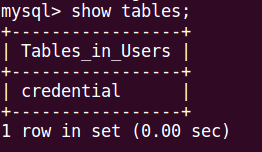
\includegraphics[width=0.3\linewidth]{show-tables}\\
\end{center}
Now I can see that there is a table in users called credentials. But I'll want to know what columns it has in order to select any data out of it.
\begin{lstlisting}[language=sh]
mysql> describe credential;
\end{lstlisting}
This will tell me what columns the table has, and some more information about each column such as its type, default value and some other info. It will look like this:\\
\begin{center}
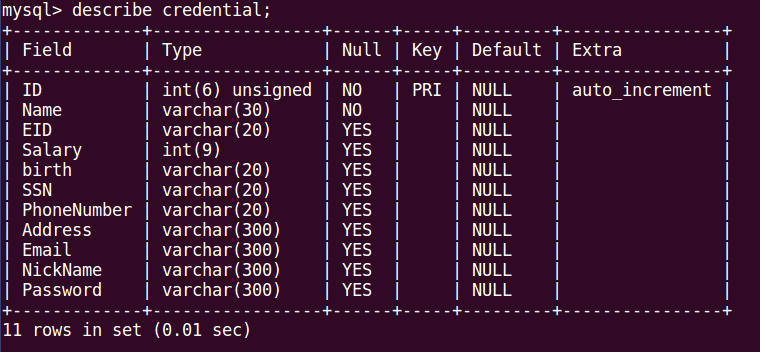
\includegraphics[width=\linewidth]{describe-credential}\\
\end{center}
Now I can formulate a query to retrieve all the information for an employee named Alice. This Query will look like this
\begin{lstlisting}[language=sh]
SELECT * FROM credential where Name="Alice";
\end{lstlisting}
And the output will look as follows:\\
\begin{center}
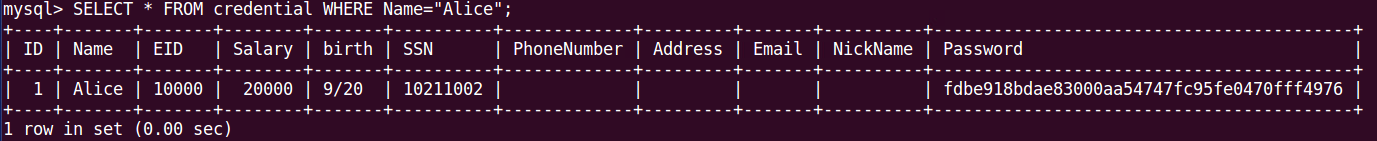
\includegraphics[width=\linewidth]{select-alice-credential}\\
\end{center}


\section{Task 2: Attack with SELECT statement}
The web application for this lab starts by showing a login screen. This screen requires a username and password to authenticate the users\cite{seed-sqlatk}.\\
\begin{center}
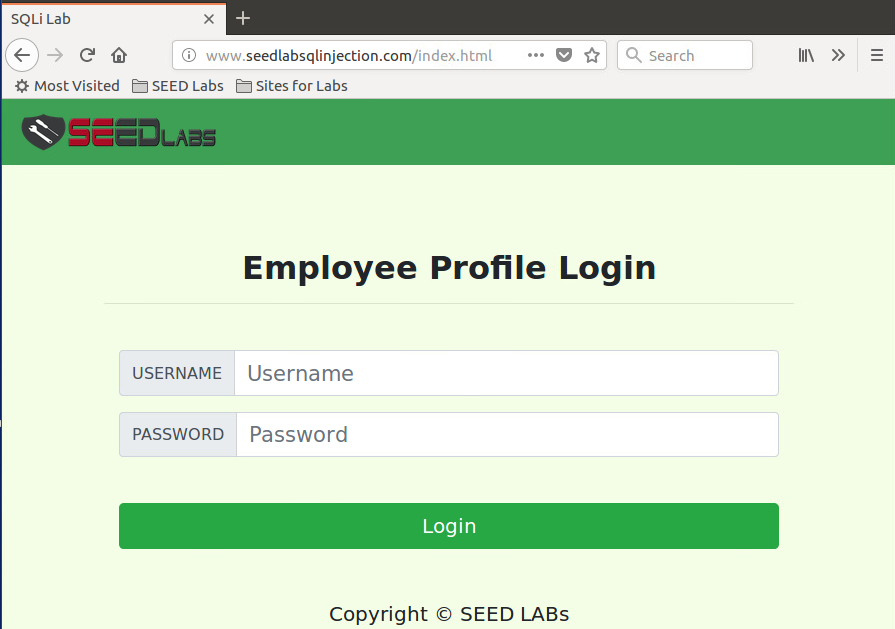
\includegraphics[width=\linewidth]{home-page}\\
\end{center}
But with SQL injection, I can bypass this authentication. The code that has the vulnerability is unsafe\_home.php and it looks similar to this\cite{seed-sqlatk}:
\begin{lstlisting}[language=php]
// select input data from the GET array
$input_uname = $_GET['username'];
$input_pwd = $_GET['Password'];
// hash the password input
$hashed_pwd = sha1($input_pwd);
// connect to the db (this won't change later, so I'll leave it out)
...
// Create a sql statement with raw input data and the hashed password field
$sql = "SELECT id, name, eid, salary, birth, ssn, address, email,
nickname, Password
FROM credential
WHERE name= '$input_uname' and Password='$hashed_pwd'";
// submit the query to the database.
$result = $conn -> query($sql);
// The following is Pseudo Code
// see if a user was returned
if(id != NULL) {
	// if a user was returned, determine if it is an admin or regular user
	if(name=='admin') {
		return All employees information;
	} else if (name !=NULL){
		return employee information;
	}
} else {
	Authentication Fails;
}
\end{lstlisting}

The query in this code select the user's id, name, eid, salary, birth, ssn, address, email, nickname, and password. And it is selecting this information for the user who's name matches the given username, and who's password matches the sha1 hash of the given password. This code takes the given username from the get array, and places it directly in the SQL statement. This means that the data is unfiltered and can be easily injected with malicious code.  If the SQL query returns a user who is of named admin, it will return a table of all employee information, and will otherwise return only the single employee's information\cite{seed-sqlatk}.


\subsection{njection attack from webpage}
Now I need to login to the web application as the administrator so that I can see of the employee's information. I can assume the administrator's name is admin (a common naming for administrator accounts, and supported by code). I will need to bypass the password field since I do not know it. To bypass the password, I need to remove that last part of the sql statement so that the query will only look for user accounts based on only the username. I can cut off the end of a sql statement by starting a comment using the -- (double dash) or \# (hash) symbols. This will tell mysql that the rest of the query is a comment, and thus should be ignored.
Since the php code is placing the username inside of a string in the SQL Query, I will need to close the string by hand and start the comment after the closing quotation mark. So the Injection code will like this
\begin{lstlisting}[language=sh]
admin' --
\end{lstlisting}
This will make the query's where clause look as follows:
\begin{lstlisting}[language=sh]
WHERE name='Admin' -- and Password='<hash of password field>';
\end{lstlisting}
\begin{center}
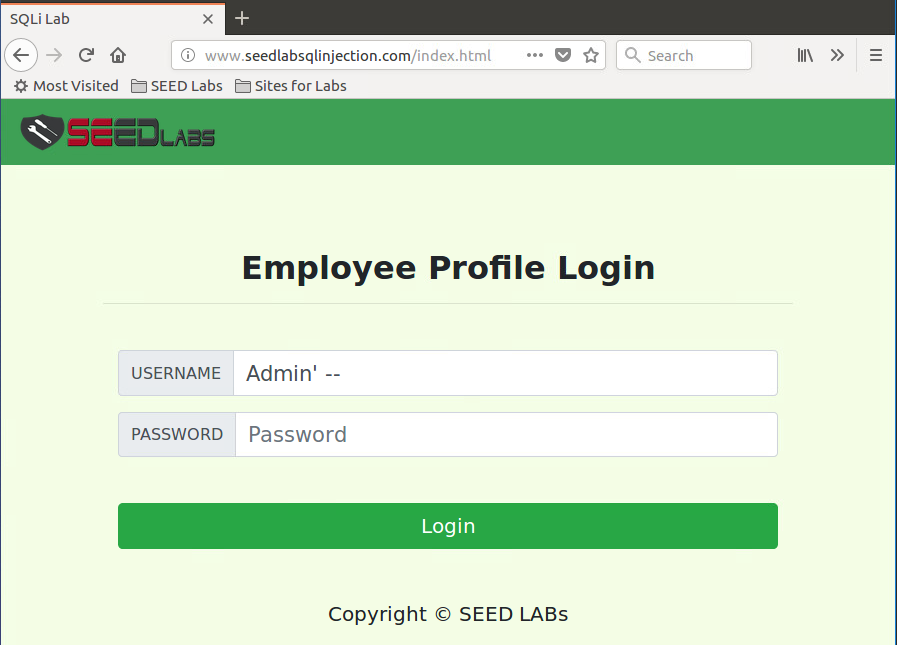
\includegraphics[width=\linewidth]{home-page-filled}\\
\end{center}
This will tell mysql that we want the user who's username is Admin, and we don't care about the password. After entering the injection code, the website returns successfully with:\\
\begin{center}
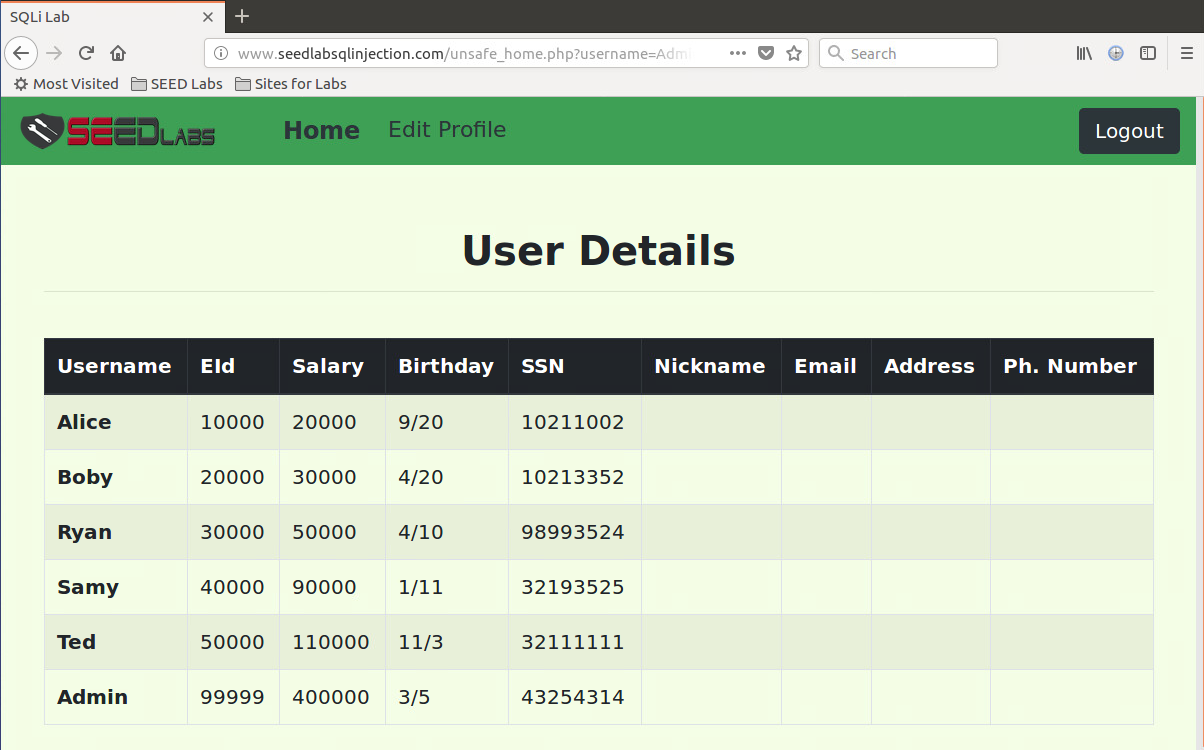
\includegraphics[width=\linewidth]{unsafe_home-admin}\\
\end{center}
It looks like the attack was successful, and I was able to retrieve the admin page that contains all of the employee's data. I can use this same attack later to login as any other user by replacing the admin username with another employee's username.

\subsection{Injection attack from command line}

For this task I will essentially do the same attack, but from the command line. Since I will not be able to use the input boxes to format the url get array for me, I will need to add the parameters as url query elements.
Since curl requires the username value to be url encoded, I have to switch spaces to +, quotation marks to \%27, and \# to \%23 \cite{seed-sqlatk}.
These changes make
\begin{lstlisting}[language=sh]
admin' #
\end{lstlisting}
To look like
\begin{lstlisting}[language=sh]
admin%27+%23+
\end{lstlisting}
By giving these values through the url, the website will be able to retrieve the input from the get array in php. This will look like:
\begin{lstlisting}[language=sh]
curl 'www.seedlabsqlinjection.com/unsafe_home.php?username=admin%27+%23+&Password='
\end{lstlisting}
when this command returns, it gives the html of the admin's page, which means that the sql attack was successful.

\subsection{Append a new SQL statement}
From the above attacks, I can only select information from the database, but if I want to modify the database, I'll need to make a new statement that will use the update or delete command. Since I can't remove the first select part of the query, I will need to add the new query between the select statement and the comment of the rest of the query\cite{seed-sqlatk}. To end the first query (the select query) I can use a semicolon (;) to signify the end. After a semicolon I can start a second query to be executed next. I will attempt to delete a row from the database where the username is Ted. My injection code will look as follows:
\begin{lstlisting}[language=sh]
admin'; DELETE FROM credential WHERE Name='Ted' #
\end{lstlisting}
This command doesn't work in php7's mysqli by default since the mysqli\_query function does not set the connection flag for multi queries upon connection to the database server\cite{phpmultiquery}. This is set by default for security measures, but can be deactivated in php if a developer requires subqueries.

\section{Task 3: Attack with UPDATE statement}
The update statement will allow at attacker to change data in the database, which could prove to be very destructive. In this task I will be logged in as the user boby. I will be using the unsafe\_edit\_backend.php page as a way to inject my sql code into an update statement. Because in order to change the information for an employee an sql update query is needed\cite{seed-sqlatk}.

\subsection{Modify your own salary}
As the employee Alice, I am able to edit my own information in the web application. Currently my salary as the user Alice is 20000\cite{seed-sqlatk}. This edit page allows me to update my nickname, email, address, phone number, and password. So currently I'm not able to freely edit my salary using the input boxes. However with an some injected SQL code I can tell the update query to change my salary along with my other fields. I won't be able to end my sql injection with a comment since I still need to run the WHERE clause at the end of the update command. So my injection code will need to:
\begin{enumerate}
	\item Place an actual value for the given field (or leave it blank)
	\item Start a new field and supply it with a value to be changed to
	\item And finally, it will need to end in a way that does not break the query for the next input field.
\end{enumerate}
I will place my injection code in the nickname field (the first input box). So it will need to start with a nickname to be set. Then I will tell it to change the salary field in the database to be 999999, and finally I will need to finish without an ending single quote so I don't break the rest of the query. So my injection code will look like this:
\begin{lstlisting}[language=sh]
Alice', salary='999999
\end{lstlisting}
\begin{center}
	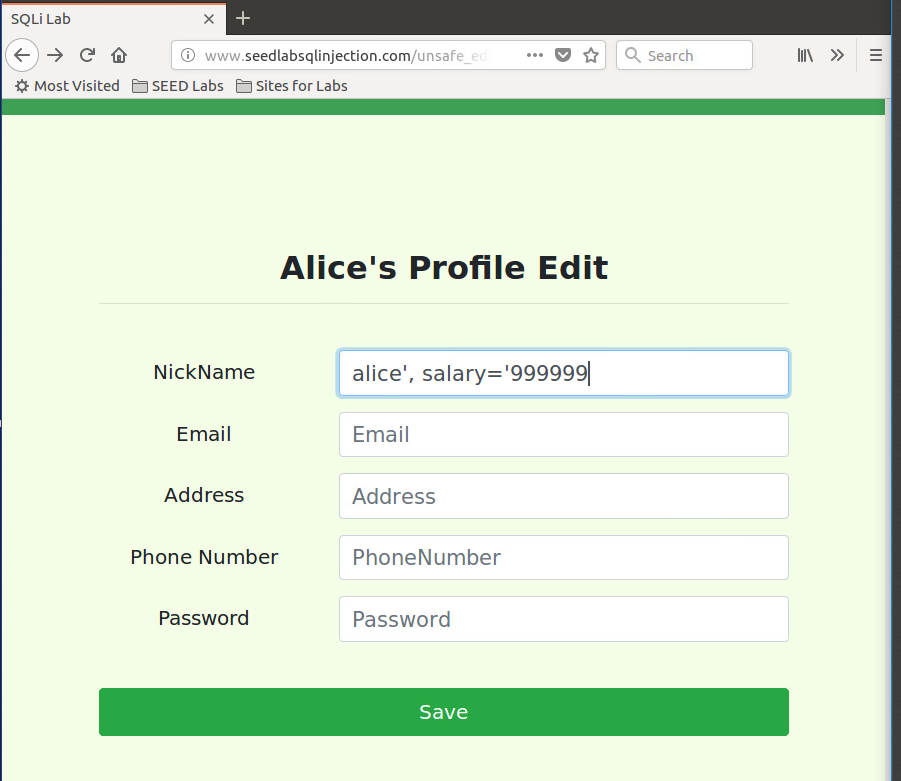
\includegraphics[width=0.6\linewidth]{alice-editing}\\
\end{center}
After running this query, I will need to go back to the home page to view the changes. The query successfully changes Alice's salary to 999999\\
\begin{center}
	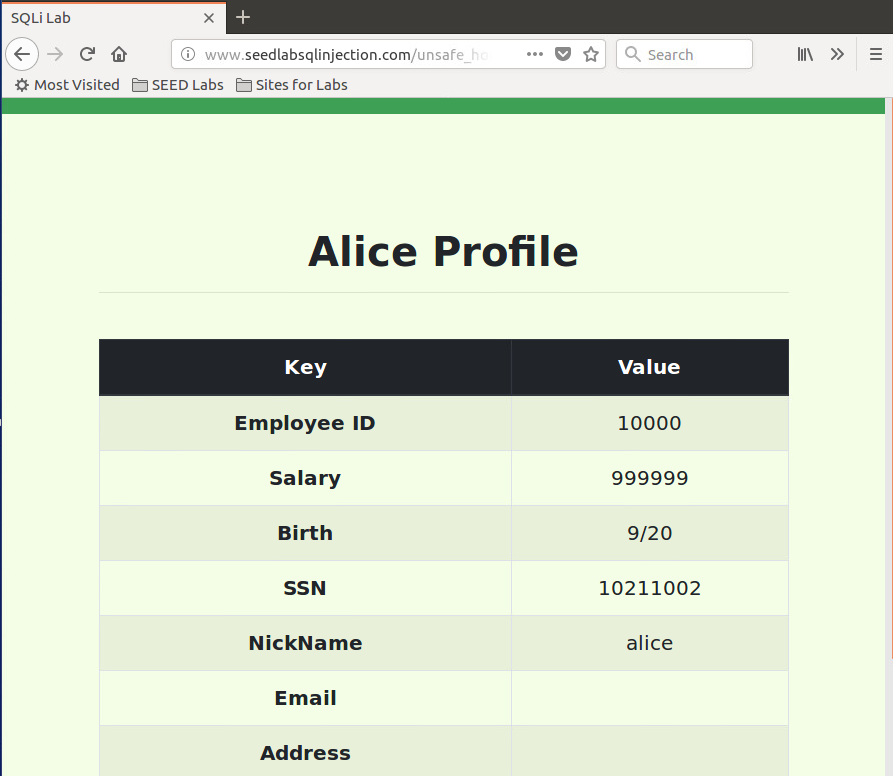
\includegraphics[width=0.6\linewidth]{alice-changed}\\
\end{center}

\subsection{Modify other people's salary}
As the user Alice, I can change more than just my information, I can change the update statement to also change other user's data if I change the user that is being edited\cite{seed-sqlatk}. \\
\begin{center}
	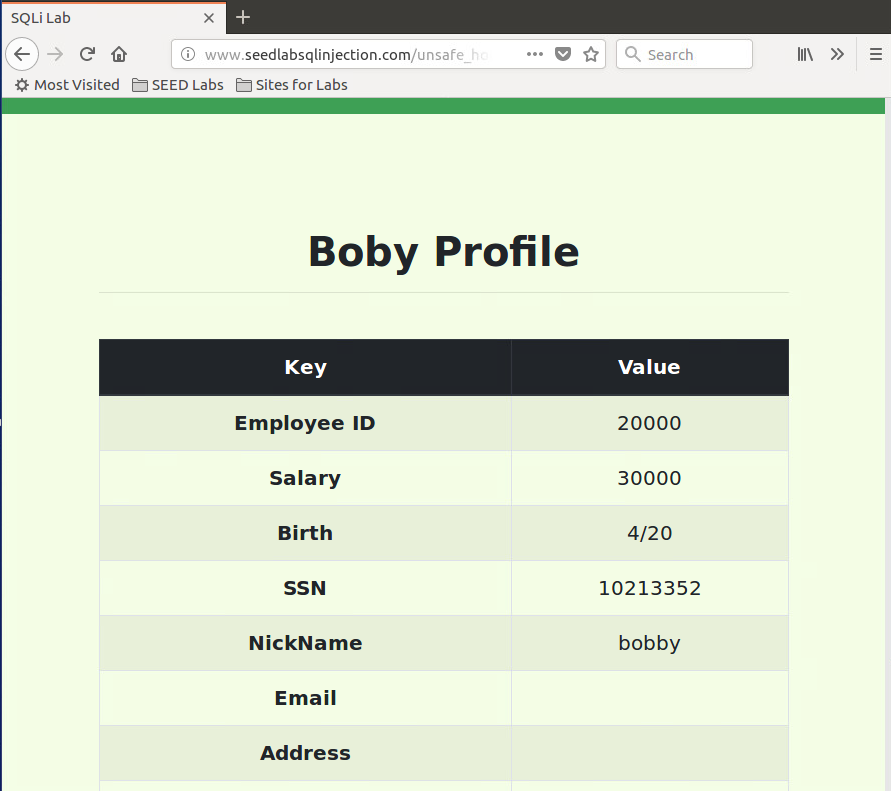
\includegraphics[width=0.6\linewidth]{boby-start}\\
\end{center}
For this task I will set boby's salary to 1 without switching users from Alice. Since the database row that is updated by the edit page is selected from the employee id number, which is set in the where clause, I will need to change the where clause to use the employee id of boby. To do this I can follow a similar exploit as the last task, but I will need to add on my own WHERE clause and comment out the rest of the query. This will look something like this:
\begin{lstlisting}[language=sh]
bobby', salary='1' WHERE EID=20000;#
\end{lstlisting}
\begin{center}
	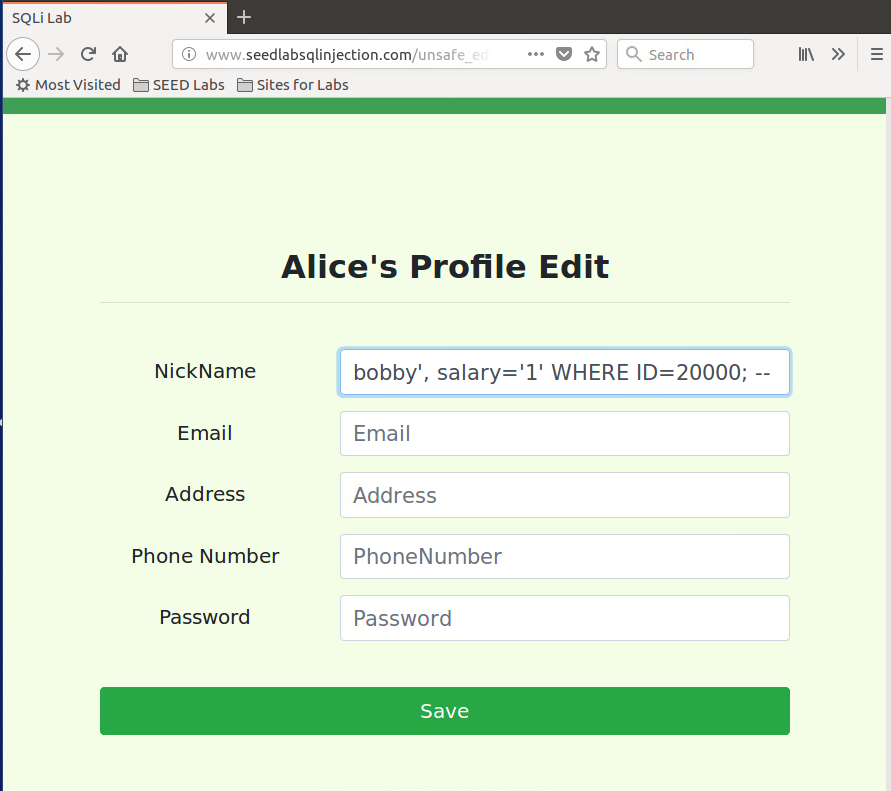
\includegraphics[width=0.6\linewidth]{alice-editing-boby}\\
\end{center}
This injection code successfully set Boby's salary to 1. So the query successfully manipulated the update query from changing the current user's basic information to editing another users private information.\\
\begin{center}
	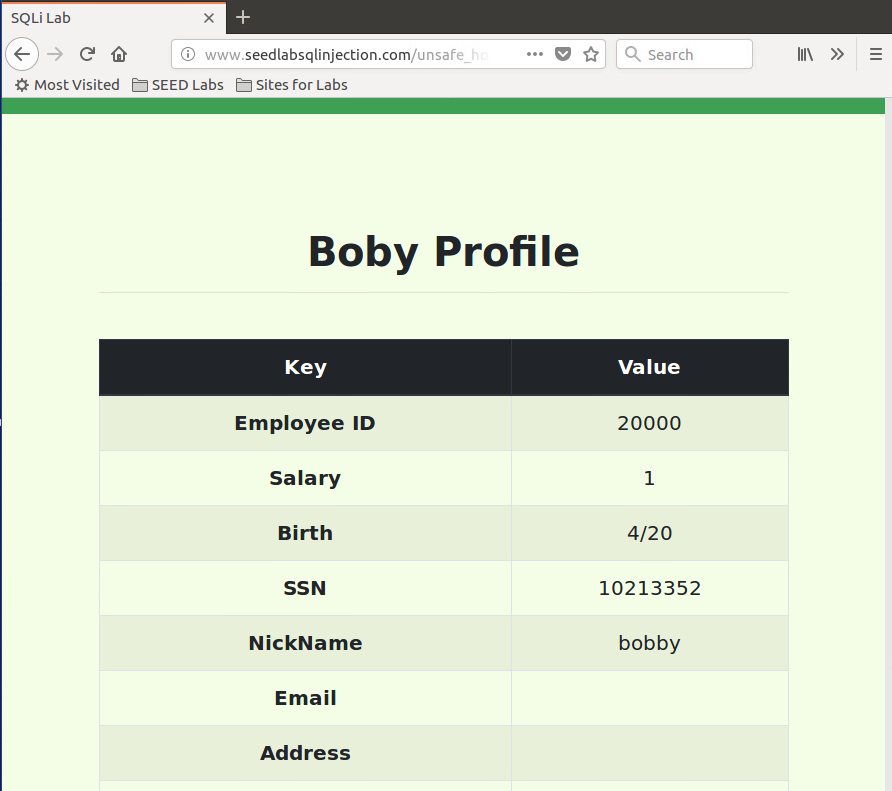
\includegraphics[width=0.6\linewidth]{alice-changed-boby}\\
\end{center}

\subsection{Modify other people's password}
Now that I have demonstrated how to edit Boby's salary, I can use a similar injection code to change his password to a specific string. In the database the password is hashed using the SHA1 hash algorithm. So if I want to be able to use the changed password that I submit, I'll need to encrypt the plain text password using sha1 before submitting it into the database\cite{seed-sqlatk}. I could do this encryption before setting the password into the query, or I could utilize mysql's built in sha1 function. I'll setup my injection code to use mysql's built in function, so I don't have to determine the sha1 hash beforehand. My query will look like this:
\begin{lstlisting}[language=sh]
Bobby', Password=SHA1('password') WHERE EID=20000;#
\end{lstlisting}
My query successfully worked and I was able to login to Boby's account using the password 'password'.

\section{Task 4: Prepared statement countermeasure}
In the attacks above, the main vulnerability is created by failure to escape input data properly. This allows an attacker almost direct access to run commands in the database system. To prevent this vulnerability, the developer needs to escape incoming data, and prepare statements before data is added. The main counter measure this lab covers is the use of prepared statements. Prepared statements go through a few phases before they are sent to the database system. First the statements are tested for syntactical errors before continuing in the process. Prepared statements are then compiled and normalized before the input data is placed in the query. In the compile phase the query is broken down to machine language and analyzed to determine what actions the query will be expected to do, such as update, delete, select, etc. Once it is in machine language, the query will be optimized to run in the best way. After the statement has gone through these phases it is cached so data can be added to it later. When the live data is placed in the complied query, it is checked again to verify that the expected action has not changed, and then it is sent to the final phase to be executed on the database\cite{seed-sqlatk}.
Instead of the normal route of compiling statements with data, prepared statements allow data to be plugged into a pre-complied query and sent to the execution phase. This allows the data to be separated from the code of the query. So if SQL code is injected into the data, it will not be ran by the complied statement, it will be treated as plain data\cite{seed-sqlatk}.
The use of prepared statements also allows the developer to identify what type of data they expect to be input by the user. While binding input data to the prepared query the developer can signify if the data should be expected to be an integer, a string, or another type of data\cite{seed-sqlatk}. In this task I will be fixing the php code from the previous tasks by implementing the prepared statements.

\begin{lstlisting}[language=php]
// select input data from the GET array and escape the raw data
$input_uname = mysqli_real_escape_string($conn, $_GET['username']);
$input_pwd = $_GET['Password'];
// hash the password input
$hashed_pwd = sha1($input_pwd);
// connect to the db (this won't change later, so I'll leave it out)
...
// Create a sql statement and prepare it for data
$stmt = $conn->prepare("SELECT id, name, eid, salary, birth, ssn, address, email,
nickname, Password
FROM credential
WHERE name= ? and Password=?");
// insert the data into the query, both should be strings
$stmt->bind_param("ss", $input_uname, $hashed_pwd);
// submit the query to the database
$stmt->execute();
// align the returned columns with variables
$stmt->bind_result($id, $name, $eid, $salary, $birth, $ssn, $address, $email);
// get the returned row
$stmt->fetch();
// The following is Pseudo Code
// see if a user was returned
if(id != NULL) {
	// if a user was returned, determine if it is an admin or regular user
	if(name=='admin') {
		return All employees information;
	} else if (name !=NULL){
		return employee information;
	}
} else {
	Authentication Fails;
}
\end{lstlisting}
After this update to the php code, and query manipulation will be escaped and translated into data rather than being executed as code. This prevents any of the injection codes that have been used previously in this lab.
\newpage
\bibliographystyle{ACM}
\bibliography{../../citations}
\end{document}
